% This is LLNCS.DEM the demonstration file of
% the LaTeX macro package from Springer-Verlag
% for Lecture Notes in Computer Science, version 1.


%% \usepackage[T1]{fontenc}
%% \usepackage[latin9]{inputenc}
%% \usepackage{geometry}
%% \geometry{verbose,letterpaper,tmargin=5cm,bmargin=3cm,lmargin=3cm,rmargin=3cm,headheight=5cm,headsep=1cm}
%% \pagestyle{headings}
%% \usepackage{array}
%% \usepackage{verbatim}
%% \usepackage{longtable}
%% \usepackage{varioref}
%% \usepackage{float}
%% \usepackage{amsmath}
%% \usepackage{color}
%% \usepackage{graphicx}
%% \usepackage{amssymb}


\documentstyle[graphicx,amsmath,float,array]{llncs}

%
\begin{document}

\title{Parallel Transductive Linear SVM for Text Classification}

\author{Miguel Fernando Cabrera and Jairo Espinosa Oviedo}

\institute{Universidad Nacional de Colombia - Sede Medell\'{i}n,
  Medell\'{i}n, Colombia
  {\it \{mfcabrer,jespinov\}}@unal.edu.co 
}


\maketitle

\begin{abstract}
Transductive Support Vector Machines (TSVM) have shown improvements
on classification tasks such as Text Categorization (TC), where the
features present co-occurrence and the training samples are few in
comparison with the data available. Although the nature of the TSVM
algorithm as described by Joachim makes it difficult to be as fast
as a regular SVM, the parallelization of this algorithm is interesting
when the gains in classification performance are crucial. Solving
TSVM algorithm requires the solution of multiple quadratic programming
problems that generally scales to $O(n^{3})$. We describe the implementation
of a TSVM Solver for 2-class problem using a parallel architecture
which aims to improve the necessary computation times while preserving
the classification performance. This strategy produced an implementation 
that is 2x - 7x faster than a regular TSVM for a TC problem of 2,000 vectors 
and more than 30,000 features.

{\bf Keywords:} SVM, Text Classification, Machine Learning, Algorithm,
Parallel Algorithm, Information Retrieval,Artificial Intelligence

\end{abstract}



\section{Introduction}

Text classification is a key aspect of text filtering, document management
and retrieval tasks. Besides basic document classification for some
kind of digital library, many problems can be seen as instances of
the Text Categorization (TC) problem . Spam detection, Web search
improvement and automated metadata generation are just a few examples
of this \cite{Sebastiani02}.  Some of those tasks can be achieved
by human beings, but a manual classification is at best expensive
and practically impossible for large amounts of documents found today
in modern information systems.

A TC technique uses example documents that have been previously categorized
in classes by an authority in order to learn a model that, with an
associated error value, can automatically predict the class that the
authority would have given to future documents. 

Support Vector Machines \cite{Vapnik98} are powerful tools for classifying
large data sets, and due the nature of the classical text representation
models, it has been applied successfully in automated document classification
tasks \cite{Joachims98,Joachims99c}. An special type of SVM, based
on Transductive inference (TSVM), has demonstrated to be more effective
for document classification than the common inductive inference based
SVM \cite{Joachims99c}.

One characteristic of the SVM is that, in its formal definition, the
computation and memory storage requirements increase rapidly with
the number of training vectors. This is due the fact that the SVM
classification problem is a Quadratic Programming problem (QP) that
finds the support vectors in all training data set. Solvers of this
kind of problem generally scales to $O(n^{3})$ making it a very computationally
expensive problem.

%% One approach to cope with this limitation is to divide the problem
%% into chunks \cite{Joachims/99a,osunaetal97} and train those sub-problems.
%% Even with these optimizations, the problem still has large computational
%% requirements, and the required time to train grows sufficiently enough
%% for making it not useful for real-time training when using large data
%% sets. The implementation of Transductive inference for a SVM requires
%% to solve the same problem many times over generally large data sets,
%% until finding the optimal classifier. This makes the scaling problem
%% for Transductive SVM even more difficult, therefore, methods for optimizing
%% the training process need to be developed.

%% Taking advantage actual trends in processor technologies, where the
%% multi-core processor is becoming the norm \cite{Marowka07,1069628|Geer05}
%% parallel implementation of such algorithm along with other optimization
%% will help make the application of this technique practical in real
%% world situations. Also, as an extra motivation, empirical results
%% have showed that some parallel settings for SVM have achieved better
%% generalization than their classic counterparts for some problems \cite{citeulike:935557|Collobert2002}.

This paper describes an implementation of a parallel SVM with the
cascade model described in \cite{GrafCBDV04} using a Transductive
learning algorithm. 
%% The first part, Overview, introduces the basic
%% concepts a Machine Learning, Information Retrieval and Text Categorization.
%% Later we describe the SVM algorithm and justify the reason of using
%% SVM for text classification over other techniques. In chapter \ref{cha:Experiments-and-Results}
%% we exhibit our experimental set-up and the show the analysis of the
%% results.


%
\section{Models of Text and Text Representation\label{sub:Models-of-Text}}
%

Usually in a digital library database a set of words that defines
the topics or the main characteristics of a document is manually defined.
The main objective of this is to help the search of the physical document
(e.g books, papers,etc.). This list of terms or keywords enables the
user to query documents related to one or more concepts. One of the
main problems of this is that only few keywords are associated with
a defined document, and generally this assignation is made at hand,
making it expensive and error prone. Generally this querying these
systems was limited to the numbers of keywords assigned and some metadata
like title, author and dates of publication, being the user unable
to query the whole document, making the retrieval task significantly
harder.

Nowadays in digital libraries and similar systems where the all the
text is available in digital form, automatic keyword extraction makes
sense because these keywords are tightly associated with the content.
This keywords are called indexes and the task of associating each
document with a set of keywords is called \emph{indexing}. 

Indexing is based is predefined group of keywords: the dictionary
or vocabulary. As mentioned above, in a digitalized text database
(also called a corpus) the dictionary is usually extracted from the
set of words present in the corpus, and the expensive manual indexing
can be avoided by representing the documents by the dictionary terms
they are made of. Given that all the full text is available for querying
it, now problem is to find the best way of representing the text in
order to extract the more important words, that is, the keywords that
define it. 

During the last few decades many representation forms have been developed
ranging from simple word appearance binary representation to a concept
\cite{deerwester90indexing}, probabilistic \cite{keller-theme} and
even Neural Networks \cite{DBLP:conf/icann/KellerB05} based ones. 

The most common approach to automatically extract the index terms
from a corpus is called vector space model \cite{361220}. In this
model each document $d$ is represents as a vector$(\theta_{1},...,\theta_{M})$
where $\theta_{j}$ is a function of the frequency in $d$ of the
$j^{th}$ word of a chosen dictionary $M$. 

Based in this definition various forms of $\theta(j)$have been defined:

\begin{description}
\item [{Binary}] In which $\theta_{j}$ is equal to 1 if the $j^{th}$
word appears in the document or 0 otherwise.
\item [{Frequency}] In which $\theta_{j}$ is equal to the number of times
$j^{th}$ word appears in the document.
\item [{\emph{tf-idf}}] In which $\theta_{j}$ is equal to the \emph{tf-idf}
formula:
\end{description}
\begin{equation}
\theta_{j}=tf_{j}(d)\centerdot log(\frac{N}{df_{j}}),\,\,\,\,\forall j\in\{1,\ldots,M\}\label{eq:tf-idf}\end{equation}


The equation \ref{eq:tf-idf} was defined proposed by Salton and Buckley
\cite{866292} and it is the more complex of the three. the $tf_{j}(d)$
(term frequency) is the number of times that the $j^{th}$ word appears
in the document $d$, $df_{j}$ is the number of documents the term
appears in all the corpus and $N$ is the total number of documents
in the corpus. 
%% The main reason behind this formulation is that in
%% the context of document retrieval it is considered that words appearing
%% too frequently across the corpus may not be discriminant, therefore
%% this formula gives more importance to terms appearing more frequently
%% in the documents while penalizing the ones that appears in to many
%% documents. The reader may have noticed that this representation of
%% text does not take into account the actual order of the words inside
%% the document, despite this, vector space model have performed well
%% and it still used with some variations in the majority of IR systems.

the vector space model representation described above may seem simplistic
in comparison with the more complex representations mentioned first,
nevertheless, it seems that for some tasks like text categorization,
the classical tf-idf works just well and more complex representations
of the text do not significantly affect the performance of the methods.

%
\begin{figure}
\begin{centering}
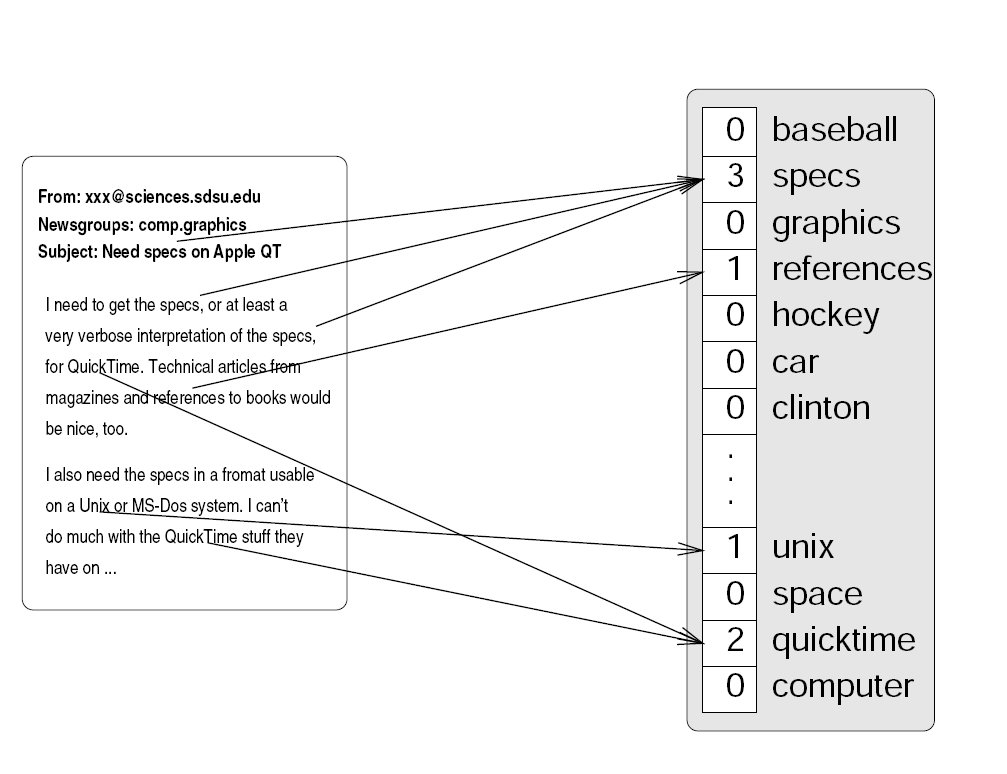
\includegraphics[scale=0.2]{images/joachims-text-vect}
\par\end{centering}

\caption{Representing text as a feature vector \cite{Joachims98}}

\end{figure}


\section{Support Vector Machines}

Support Vector Machines (SVMs) \cite{Vapnik98} are powerful classification
and regression tools that have been widely applied in the solutions
of many problem, generally yielding comparable or even better performance
that other algorithms. 

The SVM algorithm is based on the concept of VC Dimension\cite{vapnik71uniform}
and on the principle of structural risk minimization developed by
Vapnik \cite{Vapnik99,vapnik71uniform}. Roughly, the VC dimension
is a metric of how complex a classifier machine is, complex classifier
has more capacity to fit the training data, thus, overfitting is more
likely to occur, therefore, is preferred a classifier with minimum
VC Dimension. 

The basic idea of empirical risk minimization principle is to find
an hypothesis $s$ from an hypothesis space $S$ for which the lowest
probability of error is guaranteed for a given set of training examples. 

For linear classification problems this is equivalent to find the
discrimination function that maximizes the distances within the classes,
assuring the lowest probability of error\cite{citeulike:368926|Haykin1998}.
The aim of the Support Vector classification is to devise a computationally
efficient way of learning the optimal separating hyperplanes in high
dimensional feature space \cite{citeulike:114719|Cristianini2000introSVM}.


\section{SVM and Text Categorization}

The usage of SVM was first introduced by Joachims \cite{Joachims98,Joachims99c}
and similar setups have been used in posterior literature\cite{DumaisPHS98}.
the TC task using SVM can bee seen geometrically as finding an hyperplane
(decision surface) that separates two groups of points. Each point
is a vector representation of a document which can be done using any
of the models described back in section \ref{sub:Models-of-Text}.
As argued by Joachims \cite{Joachims98}, SVMs offer two important
advantages for TC:

\begin{itemize}
\item Doing term selection is generally not needed, because SVM are robust
to overfitting problems and can scale up to high dimensions.
\item No human and machine effort in parameter tuning on a validation set
is needed, as there is a theoretical default choice of parameter settings.
\end{itemize}
These two characteristics makes the SVMs attractive for tackling this
kind of problems. In real life scenarios, TC problems involves high
dimensional data and large amount of computing processing. As mentioned
before, the fact that SVM need a lot of calculation power for training
makes it an important motivation for using a parallel algorithm when
training SVM.


\section{Transductive Learning for SVM and Text Categorization\label{sub:Transductive-Learning-for}}

So far with the formulations described in the last section we are
using what is called inductive learning, in other words we start from
a set of examples, and based on them we try to find a classificator
function that classifies correctly the data. This is called Inference
learning, that is, going from particular examples to a general hypothesis.
The Transductive setting on the other hand, tries to use the known
distribution of the test data in order produce a classifier. 

This setting has a clear application when we don\textquoteright{}t
care about the particular function; we only need to classify a given
set of examples (i.e test set) with as few errors as possible. The
Transductive inference uses the training examples previously labeled
and the unclassified examples to generate an optimal partition and
labeling of the unclassified examples, using the prior knowledge provided
by the distribution of the unclassified examples.

The goal of the TSVM or Transductive learner is to select a function
$hL=L(S_{train},S_{test})$ from the hypothesis space $H$ using $S_{train}$
and $S_{test}$ such that the expected number of erroneous predictions
on the test and the training samples is minimized. But, why not use
the learning rule obtained by means of the training examples to classify
the test examples? The problem arises when a small training set is
use. The classifier will have a \textquotedblleft{}poor\textquotedblright{}
generalization due to the lack of knowledge about the distribution
of points in the space $X$. 

The classifier function estimated with very few points will lead to
disappointing results. Unlike of the inductive setting, the Transductive
setting uses the location of the test examples when defining the structure.
Such structure corresponds to a structure of possible hypothesis solution.
Using prior knowledge about the nature of testing data provides extra
information to built an appropriate structure. The structure is build
based on the margin on both the training and the test data.

The setting of transductive svm for TC was introduced by Joachims
\cite{Joachims99c}. The basic setup consists in a set of training examples: $\left\{
(\overrightarrow{x_{1}},y_{1}),(x_{2},y_{2}),...,(x_{n},y_{n})\right\}$, and each f them
consists of a document vector $\overrightarrow{x}$ 


%
\begin{figure}[H]
\begin{centering}
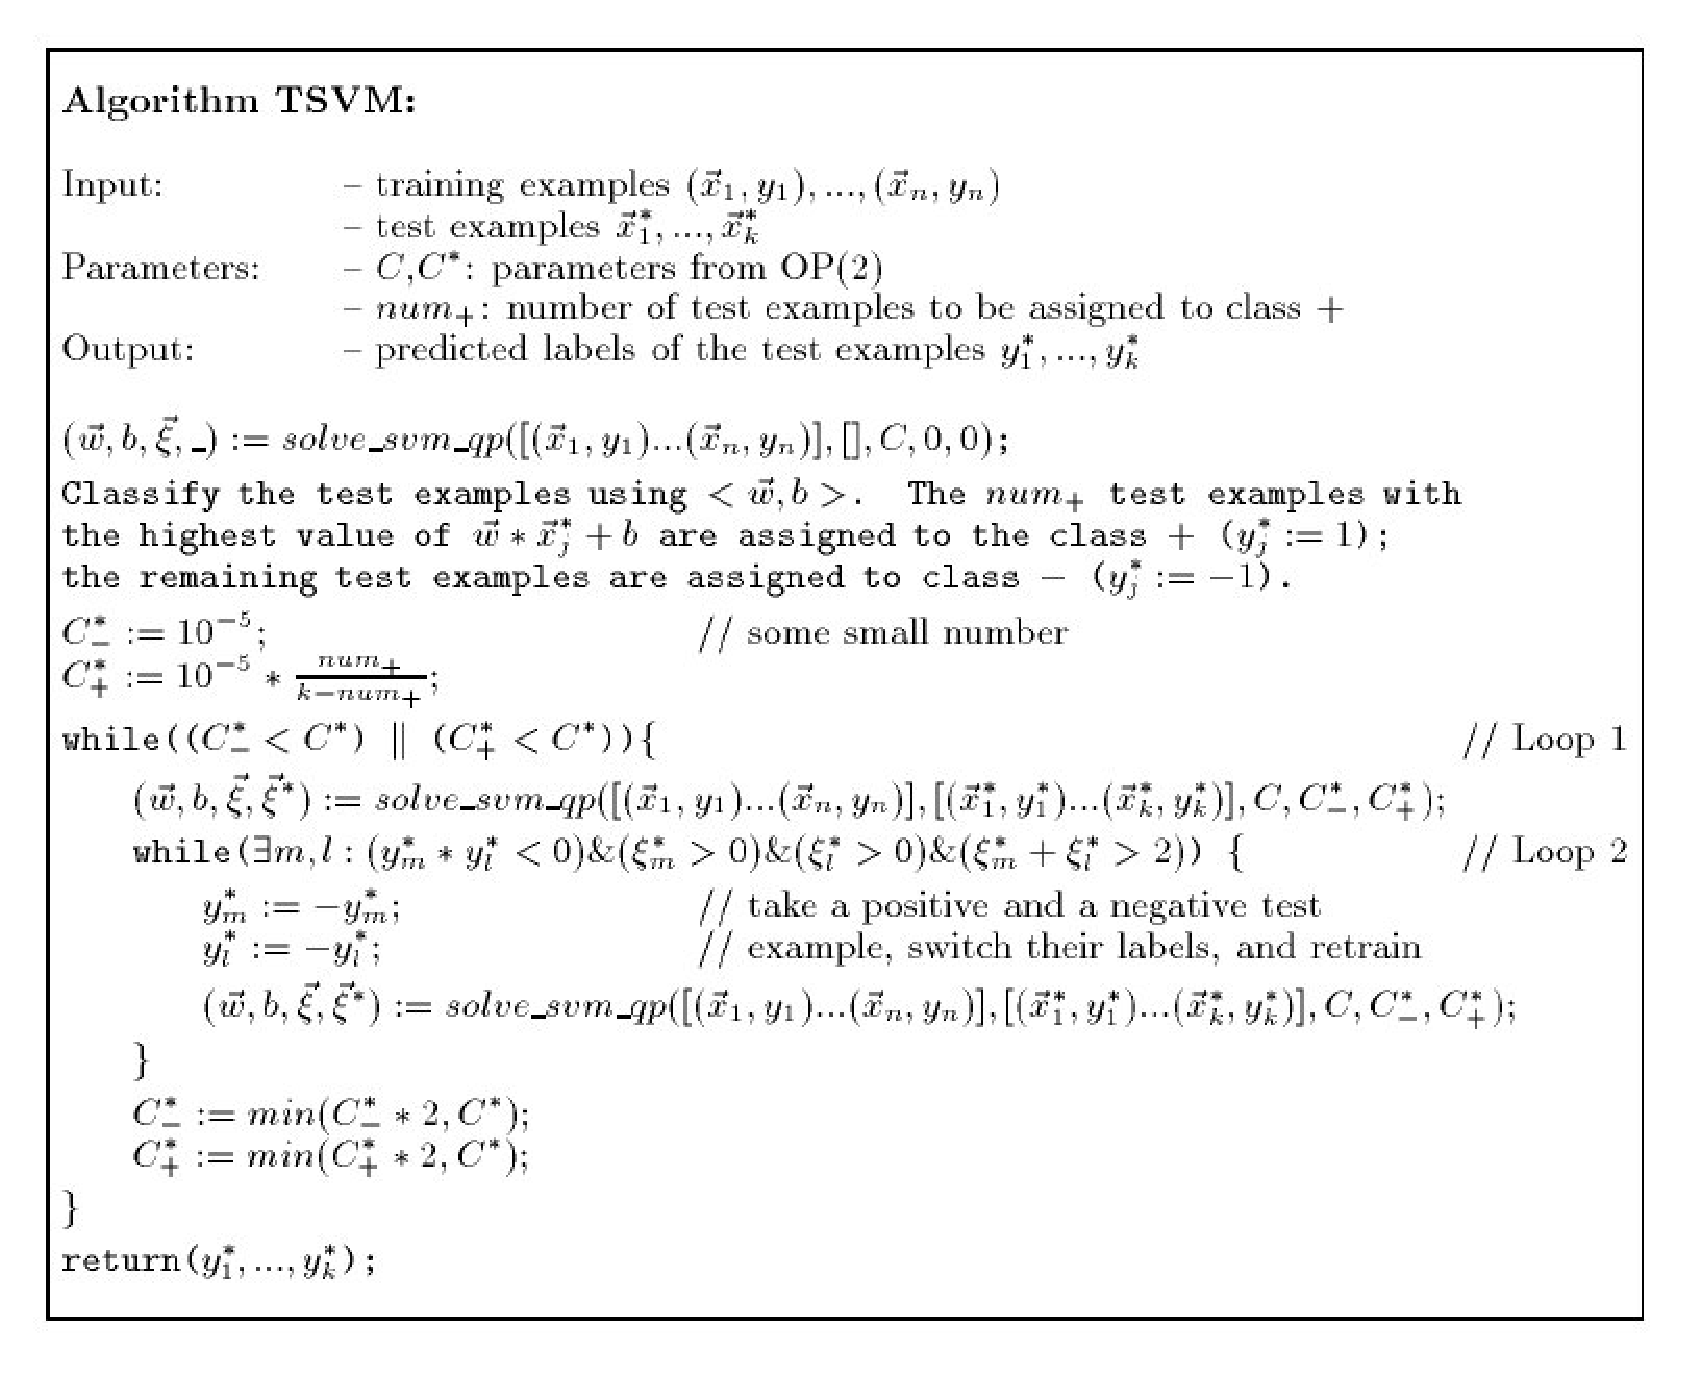
\includegraphics[scale=0.42]{images/joachims-algorithm}\label{fig:alg-tsvm}
\par\end{centering}

\caption{Algorithm for training Transductive Support Vector Machines \cite{Joachims99c}}


\end{figure}


For a complete description and a in depth study of the Joachims' approach see the nominal paper \cite{Joachims99c}
and work of Collobert \cite{1248609}.


%
\section{Fixed-Period Problems: The Sublinear Case}
%
With this chapter, the preliminaries are over, and we begin the search
for periodic solutions to Hamiltonian systems. All this will be done in
the convex case; that is, we shall study the boundary-value problem
\begin{eqnarray*}
  \dot{x}&=&JH' (t,x)\\
  x(0) &=& x(T)
\end{eqnarray*}
with $H(t,\cdot)$ a convex function of $x$, going to $+\infty$ when
$\left\|x\right\| \to \infty$.

%
\subsection{Autonomous Systems}
%
In this section, we will consider the case when the Hamiltonian $H(x)$
is autonomous. For the sake of simplicity, we shall also assume that it
is $C^{1}$.

We shall first consider the question of nontriviality, within the
general framework of
$\left(A_{\infty},B_{\infty}\right)$-subquadratic Hamiltonians. In
the second subsection, we shall look into the special case when $H$ is
$\left(0,b_{\infty}\right)$-subquadratic,
and we shall try to derive additional information.
%
\subsubsection{ The General Case: Nontriviality.}
%
We assume that $H$ is
$\left(A_{\infty},B_{\infty}\right)$-sub\-qua\-dra\-tic at infinity,
for some constant symmetric matrices $A_{\infty}$ and $B_{\infty}$,
with $B_{\infty}-A_{\infty}$ positive definite. Set:
\begin{eqnarray}
\gamma :&=&{\rm smallest\ eigenvalue\ of}\ \ B_{\infty} - A_{\infty} \\
  \lambda : &=& {\rm largest\ negative\ eigenvalue\ of}\ \
  J \frac{d}{dt} +A_{\infty}\ .
\end{eqnarray}

Theorem 21 tells us that if $\lambda +\gamma < 0$, the boundary-value
problem:
\begin{equation}
\begin{array}{rcl}
  \dot{x}&=&JH' (x)\\
  x(0)&=&x (T)
\end{array}
\end{equation}
has at least one solution
$\overline{x}$, which is found by minimizing the dual
action functional:
\begin{equation}
  \psi (u) = \int_{o}^{T} \left[\frac{1}{2}
  \left(\Lambda_{o}^{-1} u,u\right) + N^{\ast} (-u)\right] dt
\end{equation}
on the range of $\Lambda$, which is a subspace $R (\Lambda)_{L}^{2}$
with finite codimension. Here
\begin{equation}
  N(x) := H(x) - \frac{1}{2} \left(A_{\infty} x,x\right)
\end{equation}
is a convex function, and
\begin{equation}
  N(x) \le \frac{1}{2}
  \left(\left(B_{\infty} - A_{\infty}\right) x,x\right)
  + c\ \ \ \forall x\ .
\end{equation}

%
\begin{proposition}
Assume $H'(0)=0$ and $ H(0)=0$. Set:
\begin{equation}
  \delta := \liminf_{x\to 0} 2 N (x) \left\|x\right\|^{-2}\ .
  \label{eq:one}
\end{equation}

If $\gamma < - \lambda < \delta$,
the solution $\overline{u}$ is non-zero:
\begin{equation}
  \overline{x} (t) \ne 0\ \ \ \forall t\ .
\end{equation}
\end{proposition}
%
\begin{proof}
Condition (\ref{eq:one}) means that, for every
$\delta ' > \delta$, there is some $\varepsilon > 0$ such that
\begin{equation}
  \left\|x\right\| \le \varepsilon \Rightarrow N (x) \le
  \frac{\delta '}{2} \left\|x\right\|^{2}\ .
\end{equation}

It is an exercise in convex analysis, into which we shall not go, to
show that this implies that there is an $\eta > 0$ such that
\begin{equation}
  f\left\|x\right\| \le \eta
  \Rightarrow N^{\ast} (y) \le \frac{1}{2\delta '}
  \left\|y\right\|^{2}\ .
  \label{eq:two}
\end{equation}

\begin{figure}
\vspace{2.5cm}
\caption{This is the caption of the figure displaying a white eagle and
a white horse on a snow field}
\end{figure}

Since $u_{1}$ is a smooth function, we will have
$\left\|hu_{1}\right\|_\infty \le \eta$
for $h$ small enough, and inequality (\ref{eq:two}) will hold,
yielding thereby:
\begin{equation}
  \psi (hu_{1}) \le \frac{h^{2}}{2}
  \frac{1}{\lambda} \left\|u_{1} \right\|_{2}^{2} + \frac{h^{2}}{2}
  \frac{1}{\delta '} \left\|u_{1}\right\|^{2}\ .
\end{equation}

If we choose $\delta '$ close enough to $\delta$, the quantity
$\left(\frac{1}{\lambda} + \frac{1}{\delta '}\right)$
will be negative, and we end up with
\begin{equation}
  \psi (hu_{1}) < 0\ \ \ \ \ {\rm for}\ \ h\ne 0\ \ {\rm small}\ .
\end{equation}

On the other hand, we check directly that $\psi (0) = 0$. This shows
that 0 cannot be a minimizer of $\psi$, not even a local one.
So $\overline{u} \ne 0$ and
$\overline{u} \ne \Lambda_{o}^{-1} (0) = 0$. \qed
\end{proof}
%
\begin{corollary}
Assume $H$ is $C^{2}$ and
$\left(a_{\infty},b_{\infty}\right)$-subquadratic at infinity. Let
$\xi_{1},\allowbreak\dots,\allowbreak\xi_{N}$  be the
equilibria, that is, the solutions of $H' (\xi ) = 0$.
Denote by $\omega_{k}$
the smallest eigenvalue of $H'' \left(\xi_{k}\right)$, and set:
\begin{equation}
  \omega : = {\rm Min\,} \left\{\omega_{1},\dots,\omega_{k}\right\}\ .
\end{equation}
If:
\begin{equation}
  \frac{T}{2\pi} b_{\infty} <
  - E \left[- \frac{T}{2\pi}a_{\infty}\right] <
  \frac{T}{2\pi}\omega
  \label{eq:three}
\end{equation}
then minimization of $\psi$ yields a non-constant $T$-periodic solution
$\overline{x}$.
\end{corollary}
%

We recall once more that by the integer part $E [\alpha ]$ of
$\alpha \in \bbbr$, we mean the $a\in \bbbz$
such that $a< \alpha \le a+1$. For instance,
if we take $a_{\infty} = 0$, Corollary 2 tells
us that $\overline{x}$ exists and is
non-constant provided that:

\begin{equation}
  \frac{T}{2\pi} b_{\infty} < 1 < \frac{T}{2\pi}
\end{equation}
or
\begin{equation}
  T\in \left(\frac{2\pi}{\omega},\frac{2\pi}{b_{\infty}}\right)\ .
  \label{eq:four}
\end{equation}

%
\begin{proof}
The spectrum of $\Lambda$ is $\frac{2\pi}{T} \bbbz +a_{\infty}$. The
largest negative eigenvalue $\lambda$ is given by
$\frac{2\pi}{T}k_{o} +a_{\infty}$,
where
\begin{equation}
  \frac{2\pi}{T}k_{o} + a_{\infty} < 0
  \le \frac{2\pi}{T} (k_{o} +1) + a_{\infty}\ .
\end{equation}
Hence:
\begin{equation}
  k_{o} = E \left[- \frac{T}{2\pi} a_{\infty}\right] \ .
\end{equation}

The condition $\gamma < -\lambda < \delta$ now becomes:
\begin{equation}
  b_{\infty} - a_{\infty} <
  - \frac{2\pi}{T} k_{o} -a_{\infty} < \omega -a_{\infty}
\end{equation}
which is precisely condition (\ref{eq:three}).\qed
\end{proof}
%

\begin{lemma}
Assume that $H$ is $C^{2}$ on $\bbbr^{2n} \setminus \{ 0\}$ and
that $H'' (x)$ is non-de\-gen\-er\-ate for any $x\ne 0$. Then any local
minimizer $\widetilde{x}$ of $\psi$ has minimal period $T$.
\end{lemma}
%
\begin{proof}
We know that $\widetilde{x}$, or
$\widetilde{x} + \xi$ for some constant $\xi
\in \bbbr^{2n}$, is a $T$-periodic solution of the Hamiltonian system:
\begin{equation}
  \dot{x} = JH' (x)\ .
\end{equation}

There is no loss of generality in taking $\xi = 0$. So
$\psi (x) \ge \psi (\widetilde{x} )$
for all $\widetilde{x}$ in some neighbourhood of $x$ in
$W^{1,2} \left(\bbbr / T\bbbz ; \bbbr^{2n}\right)$.

But this index is precisely the index
$i_{T} (\widetilde{x} )$ of the $T$-periodic
solution $\widetilde{x}$ over the interval
$(0,T)$, as defined in Sect.~2.6. So
\begin{equation}
  i_{T} (\widetilde{x} ) = 0\ .
  \label{eq:five}
\end{equation}

Now if $\widetilde{x}$ has a lower period, $T/k$ say,
we would have, by Corollary 31:
\begin{equation}
  i_{T} (\widetilde{x} ) =
  i_{kT/k}(\widetilde{x} ) \ge
  ki_{T/k} (\widetilde{x} ) + k-1 \ge k-1 \ge 1\ .
\end{equation}

This would contradict (\ref{eq:five}), and thus cannot happen.\qed
\end{proof}
%
\paragraph{Notes and Comments.}
The results in this section are a
refined version of \cite{clar:eke};
the minimality result of Proposition
14 was the first of its kind.

To understand the nontriviality conditions, such as the one in formula
(\ref{eq:four}), one may think of a one-parameter family
$x_{T}$, $T\in \left(2\pi\omega^{-1}, 2\pi b_{\infty}^{-1}\right)$
of periodic solutions, $x_{T} (0) = x_{T} (T)$,
with $x_{T}$ going away to infinity when $T\to 2\pi \omega^{-1}$,
which is the period of the linearized system at 0.

\begin{table}
\caption{This is the example table taken out of {\it The
\TeX{}book,} p.\,246}
\vspace{2pt}
\begin{tabular}{r@{\quad}rl}
\hline
\multicolumn{1}{l}{\rule{0pt}{12pt}
                   Year}&\multicolumn{2}{l}{World population}\\[2pt]
\hline\rule{0pt}{12pt}
8000 B.C.  &     5,000,000& \\
  50 A.D.  &   200,000,000& \\
1650 A.D.  &   500,000,000& \\
1945 A.D.  & 2,300,000,000& \\
1980 A.D.  & 4,400,000,000& \\[2pt]
\hline
\end{tabular}
\end{table}
%
\begin{theorem} [(Ghoussoub-Preiss)]
Assume $H(t,x)$ is
$(0,\varepsilon )$-subquadratic at
infinity for all $\varepsilon > 0$, and $T$-periodic in $t$
\begin{equation}
  H (t,\cdot )\ \ \ \ \ {\rm is\ convex}\ \ \forall t
\end{equation}
\begin{equation}
  H (\cdot ,x)\ \ \ \ \ {\rm is}\ \ T{\rm -periodic}\ \ \forall x
\end{equation}
\begin{equation}
  H (t,x)\ge n\left(\left\|x\right\|\right)\ \ \ \ \
  {\rm with}\ \ n (s)s^{-1}\to \infty\ \ {\rm as}\ \ s\to \infty
\end{equation}
\begin{equation}
  \forall \varepsilon > 0\ ,\ \ \ \exists c\ :\
  H(t,x) \le \frac{\varepsilon}{2}\left\|x\right\|^{2} + c\ .
\end{equation}

Assume also that $H$ is $C^{2}$, and $H'' (t,x)$ is positive definite
everywhere. Then there is a sequence $x_{k}$, $k\in \bbbn$, of
$kT$-periodic solutions of the system
\begin{equation}
  \dot{x} = JH' (t,x)
\end{equation}
such that, for every $k\in \bbbn$, there is some $p_{o}\in\bbbn$ with:
\begin{equation}
  p\ge p_{o}\Rightarrow x_{pk} \ne x_{k}\ .
\end{equation}
\qed
\end{theorem}
%
\begin{example} [{\rm(External forcing)}]
Consider the system:
\begin{equation}
  \dot{x} = JH' (x) + f(t)
\end{equation}
where the Hamiltonian $H$ is
$\left(0,b_{\infty}\right)$-subquadratic, and the
forcing term is a distribution on the circle:
\begin{equation}
  f = \frac{d}{dt} F + f_{o}\ \ \ \ \
  {\rm with}\ \ F\in L^{2} \left(\bbbr / T\bbbz; \bbbr^{2n}\right)\ ,
\end{equation}
where $f_{o} : = T^{-1}\int_{o}^{T} f (t) dt$. For instance,
\begin{equation}
  f (t) = \sum_{k\in \bbbn} \delta_{k} \xi\ ,
\end{equation}
where $\delta_{k}$ is the Dirac mass at $t= k$ and
$\xi \in \bbbr^{2n}$ is a
constant, fits the prescription. This means that the system
$\dot{x} = JH' (x)$ is being excited by a
series of identical shocks at interval $T$.
\end{example}
%
\begin{definition}
Let $A_{\infty} (t)$ and $B_{\infty} (t)$ be symmetric
operators in $\bbbr^{2n}$, depending continuously on
$t\in [0,T]$, such that
$A_{\infty} (t) \le B_{\infty} (t)$ for all $t$.

A Borelian function
$H: [0,T]\times \bbbr^{2n} \to \bbbr$
is called
$\left(A_{\infty} ,B_{\infty}\right)$-{\it subquadratic at infinity}
if there exists a function $N(t,x)$ such that:
\begin{equation}
  H (t,x) = \frac{1}{2} \left(A_{\infty} (t) x,x\right) + N(t,x)
\end{equation}
\begin{equation}
  \forall t\ ,\ \ \ N(t,x)\ \ \ \ \
  {\rm is\ convex\ with\  respect\  to}\ \ x
\end{equation}
\begin{equation}
  N(t,x) \ge n\left(\left\|x\right\|\right)\ \ \ \ \
  {\rm with}\ \ n(s)s^{-1}\to +\infty\ \ {\rm as}\ \ s\to +\infty
\end{equation}
\begin{equation}
  \exists c\in \bbbr\ :\ \ \ H (t,x) \le
  \frac{1}{2} \left(B_{\infty} (t) x,x\right) + c\ \ \ \forall x\ .
\end{equation}

If $A_{\infty} (t) = a_{\infty} I$ and
$B_{\infty} (t) = b_{\infty} I$, with
$a_{\infty} \le b_{\infty} \in \bbbr$,
we shall say that $H$ is
$\left(a_{\infty},b_{\infty}\right)$-subquadratic
at infinity. As an example, the function
$\left\|x\right\|^{\alpha}$, with
$1\le \alpha < 2$, is $(0,\varepsilon )$-subquadratic at infinity
for every $\varepsilon > 0$. Similarly, the Hamiltonian
\begin{equation}
H (t,x) = \frac{1}{2} k \left\|k\right\|^{2} +\left\|x\right\|^{\alpha}
\end{equation}
is $(k,k+\varepsilon )$-subquadratic for every $\varepsilon > 0$.
Note that, if $k<0$, it is not convex.
\end{definition}
%

\paragraph{Notes and Comments.}
The first results on subharmonics were
obtained by Rabinowitz in \cite{rab}, who showed the existence of
infinitely many subharmonics both in the subquadratic and superquadratic
case, with suitable growth conditions on $H'$. Again the duality
approach enabled Clarke and Ekeland in \cite{clar:eke:2} to treat the
same problem in the convex-subquadratic case, with growth conditions on
$H$ only.

Recently, Michalek and Tarantello (see \cite{mich:tar} and \cite{tar})
have obtained lower bound on the number of subharmonics of period $kT$,
based on symmetry considerations and on pinching estimates, as in
Sect.~5.2 of this article.


\bibliography{biblio}{}
\bibliographystyle{plain}

%
% ---- Bibliography ----
%
%% \begin{thebibliography}{5}
%% %
%% \bibitem {clar:eke}
%% Clarke, F., Ekeland, I.:
%% Nonlinear oscillations and
%% boundary-value problems for Hamiltonian systems.
%% Arch. Rat. Mech. Anal. {\bf 78} (1982) 315--333
%% %
%% \bibitem {clar:eke:2}
%% Clarke, F., Ekeland, I.:
%% Solutions p\'{e}riodiques, du
%% p\'{e}riode donn\'{e}e, des \'{e}quations hamiltoniennes.
%% Note CRAS Paris {\bf 287} (1978) 1013--1015
%% %
%% \bibitem {mich:tar}
%% Michalek, R., Tarantello, G.:
%% Subharmonic solutions with prescribed minimal
%% period for nonautonomous Hamiltonian systems.
%% J. Diff. Eq. {\bf 72} (1988) 28--55
%% %
%% \bibitem {tar}
%% Tarantello, G.:
%% Subharmonic solutions for Hamiltonian
%% systems via a $\bbbz_{p}$ pseudoindex theory.
%% Annali di Matematica Pura (to appear)
%% %
%% \bibitem {rab}
%% Rabinowitz, P.:
%% On subharmonic solutions of a Hamiltonian system.
%% Comm. Pure Appl. Math. {\bf 33} (1980) 609--633
%% \end{thebibliography}
%
\end{document}
